% SPDX-License-Identifier: LPPL-1.3c
% Copyright (C) 2026 Christophe Jorssen
% Author and Current Maintainer: Christophe Jorssen <christophe.jorssen@gmail.com>
% LPPL maintenance status: maintained
% This file is part of luafemm. See LICENSE and LICENSES.md for its terms.
\section{A tutorial: spheres, circular plates and finite charged cylinders}
\label{sec:tutorial-electric-axisymmetric}

Kamil has a useful drawing of a cylindrical capacitor, but now wants to teach
its spherical counterpart. Merely relabelling a planar annulus would give the
wrong capacitance. He must change the physical symmetry: a meridional section
is revolved about its vertical axis. TikZ's horizontal coordinate becomes the
radius $r\geq0$ and its vertical coordinate becomes $z$.

\luafemmexamplebegin{electric-fe-sphere}
\subsection{Turn two semicircles into a spherical capacitor}
The same electrode paths and field pics work with |problem type=axisymmetric|.
A right semicircle of radius one centimetre, closed along the axis, describes
a solid spherical electrode. A second semicircle of radius two centimetres
is held at zero potential. Its |interior=dielectric| keeps the space inside
it available to the field calculation: it describes a thin spherical shell,
not a second solid ball overlapping the first.

Kamil first collects the declarations in a native pic. His reusable style
starts with a coarse mesh. The left domain edge defaults to |xmin=0| in this
symmetry; spelling it out makes the physical half-plane especially clear.

\begin{codeexample}[setup code]
\tikzset{
  lesson spherical domain/.style={femm/electrostatic={
    model=finite elements,problem type=axisymmetric,
    xmin=0,xmax=2.4,ymin=-2.4,ymax=2.4,
    outer boundary=insulated,mesh size=.3}},
  lesson spherical electrodes/.pic={
    \draw[femm electric conductor,
      femm/electric electrode={name=inner,potential=100}]
      (0,-1) arc[start angle=-90,end angle=90,radius=1]--cycle;
    \draw[very thick,femm/electric electrode={name=outer,
        potential=0,interior=dielectric}]
      (0,-2) arc[start angle=-90,end angle=90,radius=2]--cycle;}}
\end{codeexample}

The axis closure has zero revolved area. It contributes neither an artificial
electrode surface nor a sheet charge. Inside the solid inner electrode the
potential is still fixed, including on the axis. In the dielectric, regularity
is the natural scalar-potential condition; there is no rule imposing $V=0$
on the axis. The insulated box outside the grounded shell isolates this
example from artificial exterior grounding effects.

\begin{codeexample}[width=0pt]
\begin{tikzpicture}[lesson spherical domain,
    femm/electrostatic={name=spherical coarse},scale=.85]
  \pic[transform shape] {lesson spherical electrodes};
  \begin{scope}[on background layer]
    \pic {femm electric mesh};
    \pic[femm/electric={lines per charge=14}] {femm electric field};
  \end{scope}
  \draw[->] (0,-2.5)--(0,2.7) node[above] {$z$};
  \draw[->] (0,0)--(2.7,0) node[right] {$r$};
  \path[femm/electric profile={name=spherical coarse radial,samples=81}]
    (1.02,0)--(1.98,0);
\end{tikzpicture}
\end{codeexample}

The drawing shows one meridional half-plane, not a flat charged semicircle.
Rotating it through a full turn gives the physical capacitor. A display scale
or rotation changes the drawing but not this symmetry. The |transform shape|
option makes the native physical pic follow that display transformation.

\subsection{Compare the field and the total charge}
Once the geometry is satisfactory Kamil decreases |mesh size|. Curved paths
are flattened with |curve tolerance|, independently of the requested element
size. Both approximations matter near a curved electrode. Refining profile
samples or equipotential levels cannot improve the solved potential.

\begin{codeexample}[width=0pt]
\begin{tikzpicture}[lesson spherical domain,femm/electrostatic={
    mesh size=.12,name=spherical fine},scale=.85]
  \pic[transform shape] {lesson spherical electrodes};
  \begin{scope}[on background layer]
    \pic[femm/electric={lines per charge=18}] {femm electric field};
    \pic[femm/electric={levels={10,25,50,75,90}}] {femm equipotentials};
  \end{scope}
  \draw[densely dashed,gray] (0,-2.3)--(0,2.3);
  \node[above] at (1.5,2) {$V_{\rm inner}=100\,\mathrm V$};
  \path[femm/electric profile={name=spherical fine radial,samples=121}]
    (1.02,0)--(1.98,0);
\end{tikzpicture}
\end{codeexample}

For $a=1\,\mathrm{cm}$, $b=2\,\mathrm{cm}$ and $U=100\,\mathrm V$,
\[
 C=4\pi\epsilon_0\frac{ab}{b-a},\qquad
 E_r(r)=\frac{Uab}{(b-a)r^2}.
\]
In the following PGFPlots expression $x$ is measured in centimetres, so the
analytical field is $20000/x^2$ in volts per metre. |Er| and |abscissa=r|
are explicit aliases for the radial component and model-coordinate radius.
The short flat pieces are the raw P1 element fields; they are not a plotting
fault and have not been silently smoothed.

\begin{codeexample}[width=0pt]
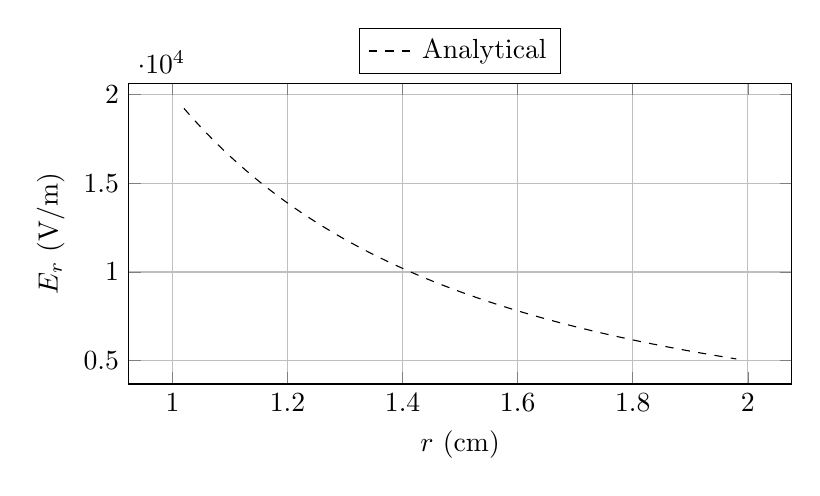
\begin{tikzpicture}
\begin{axis}[width=10cm,height=5.4cm,no markers,grid=major,
    xlabel={$r$ (cm)},ylabel={$E_r$ (V/m)},
    legend style={at={(.5,1.03)},anchor=south,legend columns=3}]
  \addplot[black,dashed,domain=1.02:1.98,samples=101] {20000/x^2};
  \addlegendentry{Analytical}
  \femmelectricplot[profile=spherical coarse radial,component=Er,abscissa=r,
    plot options={gray,thick}]
  \addlegendentry{Coarse}
  \femmelectricplot[profile=spherical fine radial,component=Er,abscissa=r,
    plot options={blue!70!black,thick}]
  \addlegendentry{Fine}
\end{axis}
\end{tikzpicture}
\end{codeexample}

Charge and energy now refer to the \emph{whole body of revolution}. There is
no extrusion depth. The theoretical inner-electrode charge is approximately
$2.2253\times10^{-10}\,\mathrm C$. The computed values below include faceting
and mesh error; comparing them is more informative than printing many digits.

\begin{codeexample}[width=0pt]
\begin{tabular}{lr}
Calculation & Inner electrode charge (C)\\
Coarse & \femmelectricvalue[model=spherical coarse,electrode=inner,
  quantity=charge]\\
Fine & \femmelectricvalue[model=spherical fine,electrode=inner,
  quantity=charge]\\
\end{tabular}
\end{codeexample}
\luafemmexampleend{electric-fe-sphere}

\luafemmexamplebegin{electric-fe-disks}
\subsection{Choose a dielectric, then let the circular plates fringe}
Kamil next returns to a capacitor with two circular plates. A horizontal
segment from the axis to radius $R$ represents a disk. He puts PTFE in the
gap with a catalogue choice and makes that declaration a reusable TikZ style.
The FEMM catalogue provides nominal permittivities, not measured values for
his particular specimen. Here |material=ptfe| selects $\epsilon_r=2$.

\begin{codeexample}[setup code]
\tikzset{lesson PTFE/.style={fill=blue!10,draw=blue!40!black,
    femm/electric region={material=ptfe}}}
\end{codeexample}

The slab reaches radius one centimetre; air surrounds its outside edge.
The box is deliberately finite and grounded. Its influence must be checked
by a separate enlargement after mesh convergence. The midplane seed contour distributes lines through the gap and the surrounding
air. The horizontal end of each
ideal zero-thickness disk is a singular edge: a largest element field is not
a converged physical maximum.

\begin{codeexample}[width=0pt]
\begin{tikzpicture}[femm/electrostatic={model=finite elements,
    problem type=axisymmetric,xmax=2.5,ymin=-1.7,ymax=1.7,
    mesh size=.14,name=PTFE disks}]
  \draw[lesson PTFE] (0,-.3) rectangle (1,.3);
  \draw[very thick,femm/electric electrode={name=upper,potential=50}]
    (0,.3)--(1,.3);
  \draw[very thick,femm/electric electrode={name=lower,potential=-50}]
    (0,-.3)--(1,-.3);
  \path[femm/electric seeds={samples=21}] (.05,0)--(2.3,0);
  \pic {femm electric field};
  \pic[femm/electric={levels={-40,-20,0,20,40}}] {femm equipotentials};
  \draw[gray,densely dotted] (0,-1.7) rectangle (2.5,1.7);
  \node[right] at (1.5,1.2) {Air};
  \node[fill=white,inner sep=1pt] at (.5,0) {PTFE};
  \path[femm/electric profile={name=disk midplane,samples=121}]
    (0,0)--(2.3,0);
\end{tikzpicture}
\end{codeexample}

The $z$ component is negative between the plates because the upper plate is
positive. A jump at the edge of the dielectric is allowed: tangential $E$
and normal $D$ obey different interface conditions. The plot preserves the
discontinuous raw field. The styles and catalogue work unchanged in a planar
calculation; only the physical interpretation and integration weights differ.

\begin{codeexample}[width=0pt]
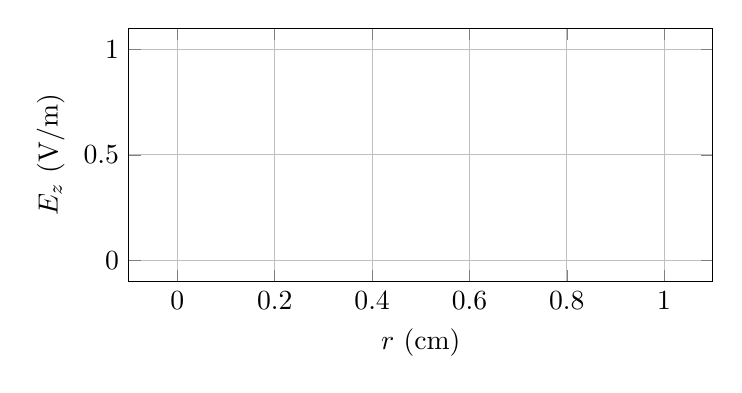
\begin{tikzpicture}
\begin{axis}[width=9cm,height=4.8cm,no markers,grid=major,
    xlabel={$r$ (cm)},ylabel={$E_z$ (V/m)}]
  \femmelectricplot[profile=disk midplane,component=Ez,abscissa=r,
    plot options={blue!70!black,thick}]
\end{axis}
\end{tikzpicture}
\end{codeexample}

Ordinary PGF order applies: |material=ptfe,relative permittivity=2.2| supplies
an explicit custom value after the catalogue default. In the reverse order,
selecting PTFE resets that value to two. Reusable styles follow the same rule.
\luafemmexampleend{electric-fe-disks}

\luafemmexamplebegin{electric-fe-bodies}
\subsection{Distinguish prescribed charges from conducting electrodes}
Finally Kamil wants a uniformly charged sphere. He replaces the inner
electrode by a dielectric region with prescribed volume density. A surrounding
grounded spherical shell supplies an unambiguous potential reference. It also
makes comparison with the analytical spherical field possible without a
rectangular far-boundary approximation.

\begin{codeexample}[width=0pt]
\begin{tikzpicture}[femm/electrostatic={model=finite elements,
    problem type=axisymmetric,xmin=0,xmax=2.4,ymin=-2.4,ymax=2.4,
    outer boundary=insulated,
    mesh size=.16,name=charged sphere FE},scale=.85]
  \draw[femm charged body,femm/electric region={volume charge density=1e-7}]
    (0,-1) arc[start angle=-90,end angle=90,radius=1]--cycle;
  \draw[thick,femm/electric electrode={name=shell,potential=0,
      interior=dielectric}]
    (0,-2) arc[start angle=-90,end angle=90,radius=2]--cycle;
  \path[femm/electric seeds={samples=17}]
    (0,-.7) arc[start angle=-90,end angle=90,radius=.7];
  \pic {femm electric field};
  \pic[femm/electric={levels={.02,.05,.1,.2,.3}}] {femm equipotentials};
  \draw[gray,densely dashed] (0,-2.2)--(0,2.2);
  \path[femm/electric profile={name=charged sphere radial,samples=121}]
    (0,0)--(1.9,0);
\end{tikzpicture}
\end{codeexample}

Inside the sphere $E_r=\rho r/(3\epsilon_0)$; outside it
$E_r=\rho R^3/(3\epsilon_0r^2)$. The shell changes the additive potential
reference, not these fields. A charged surface would instead use
|femm/electric charge layer| and |surface charge density| on the semicircle.
It prescribes $\sigma$, whereas an electrode prescribes $V$ and its charge
redistributes as required. These two physical models must not be confused.

\begin{codeexample}[width=0pt]
\begin{tikzpicture}[femm/electrostatic={model=finite elements,
    problem type=axisymmetric,xmin=0,xmax=2.4,ymin=-2.4,ymax=2.4,
    outer boundary=insulated,
    mesh size=.16,name=charged shell FE},scale=.85]
  \draw[femm charged surface,
    femm/electric charge layer={surface charge density=1e-9}]
    (0,-1) arc[start angle=-90,end angle=90,radius=1]--cycle;
  \draw[thick,femm/electric electrode={potential=0,interior=dielectric}]
    (0,-2) arc[start angle=-90,end angle=90,radius=2]--cycle;
  \path[femm/electric seeds={samples=17}]
    (0,-1.15) arc[start angle=-90,end angle=90,radius=1.15];
  \pic {femm electric field};
  \pic[femm/electric={levels={.02,.05,.1,.2,.4}}] {femm equipotentials};
  \draw[gray,densely dashed] (0,-2.2)--(0,2.2);
\end{tikzpicture}
\end{codeexample}

A rectangle touching the axis gives a finite cylinder, including its end
effects. In the next drawing the \emph{lateral surface only} carries a uniform
charge; the end caps are uncharged. To charge the entire closed surface, the
physical path would also include the two horizontal cap segments. Their
surface areas are weighted automatically, and an axis closure adds no charge.

\begin{codeexample}[width=0pt]
\begin{tikzpicture}[femm/electrostatic={model=finite elements,
    problem type=axisymmetric,xmax=3,ymin=-3,ymax=3,
    mesh size=.22,name=finite charged cylinder},scale=.7]
  \draw[gray] (0,-1) rectangle (.7,1);
  \draw[femm charged surface,
    femm/electric charge layer={surface charge density=1e-9}]
    (.7,-1)--(.7,1);
  \path[femm/electric seeds={samples=15}] (.8,-1.4)--(.8,1.4);
  \pic {femm electric field};
  \pic[femm/electric={level count=8}] {femm equipotentials};
  \draw[gray,densely dotted] (0,-3) rectangle (3,3);
  \draw[->] (0,-3)--(0,3.3) node[above] {$z$};
  \draw[->] (0,0)--(3.3,0) node[right] {$r$};
\end{tikzpicture}
\end{codeexample}

The end effects are visible here, unlike in the infinite-cylinder formula.
This is still a finite grounded box. Kamil first refines the mesh at fixed
box dimensions, then enlarges the box while retaining the local resolution.
A drawing that looks smooth is not evidence that either error is negligible.
\luafemmexampleend{electric-fe-bodies}
